% chapters/chapter2/2_4_simscape.tex
% !TeX root=../../main.tex

\section{پیاده‌سازی مدل فیزیکی در محیط \lr{Simscape}}

جهت اعتبارسنجی معادلات ریاضی و فراهم آوردن یک بستر فیزیکی (\lr{Plant}) دقیق برای بررسی الگوریتم‌های کنترلی، سیستم جرثقیل در نرم‌افزار \lr{Simscape Multibody} شبیه‌سازی شد. در این مدل، به منظور تطابق کامل دینامیک سیستم با معادلات تحلیلی، درجات آزادی متغیر با زمان (\lr{Reel Rate}) از طریق یک معماری ساختاریافته مدل‌سازی شده‌اند.

\begin{figure}[htbp]
    \centering
    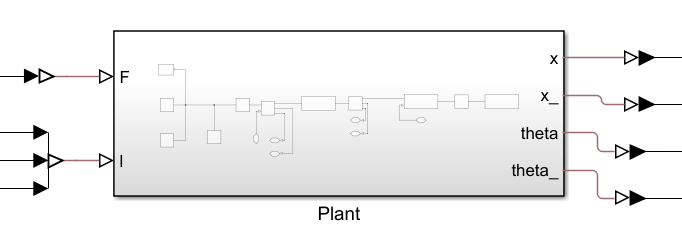
\includegraphics[width=0.75\textwidth]{images/0_System_Modeling/simscape_multibody_plant.png}
    \caption{نمای کلی بلوک \lr{Plant} سیستم جرثقیل در محیط سیمیولینک}
    \label{fig:simscape_plant}
\end{figure}

\subsection{معماری مفاصل و درجات آزادی}

ساختار فیزیکی سیستم بر پایهٔ سه مفصل اصلی توسعه یافته است:
\begin{itemize}
    \item \textbf{مفصل ارابه (\lr{X-Translation}):} حرکت افقی ارابه بر روی ریل توسط یک مفصل کشویی (\lr{Prismatic Joint}) متصل به مرجع لخت (\lr{World Frame}) مدل شده است. نیروی محرک افقیِ سیستم به صورت مستقیم به عنوان ورودی به این مفصل اعمال می‌شود.
    \item \textbf{مفصل آونگ (\lr{Pendulum Rotation}):} نوسان آونگ با استفاده از یک مفصل دورانی (\lr{Revolute Joint}) تعریف شده است. برای اعمال شرایط اولیهٔ مسئله، زاویهٔ اولیهٔ آونگ ($\theta_0$) در بخش اهداف حالت (\lr{State Targets}) این مفصل مقداردهی می‌شود تا از بروز تداخل در محاسباتِ حل‌گر (\lr{Solver}) طی لحظهٔ آغازین شبیه‌سازی جلوگیری گردد.
    \item \textbf{مفصل تغییر طول کابل (\lr{Reel Rate}):} برای ایجاد کابلی با طول متغیر، یک مفصل کشویی ثانویه در امتداد شعاع آونگ تعبیه شده است تا تغییرات سینماتیکی بار را به صورت دینامیکی شبیه‌سازی کند.
\end{itemize}

\begin{figure}[htbp]
    \centering
    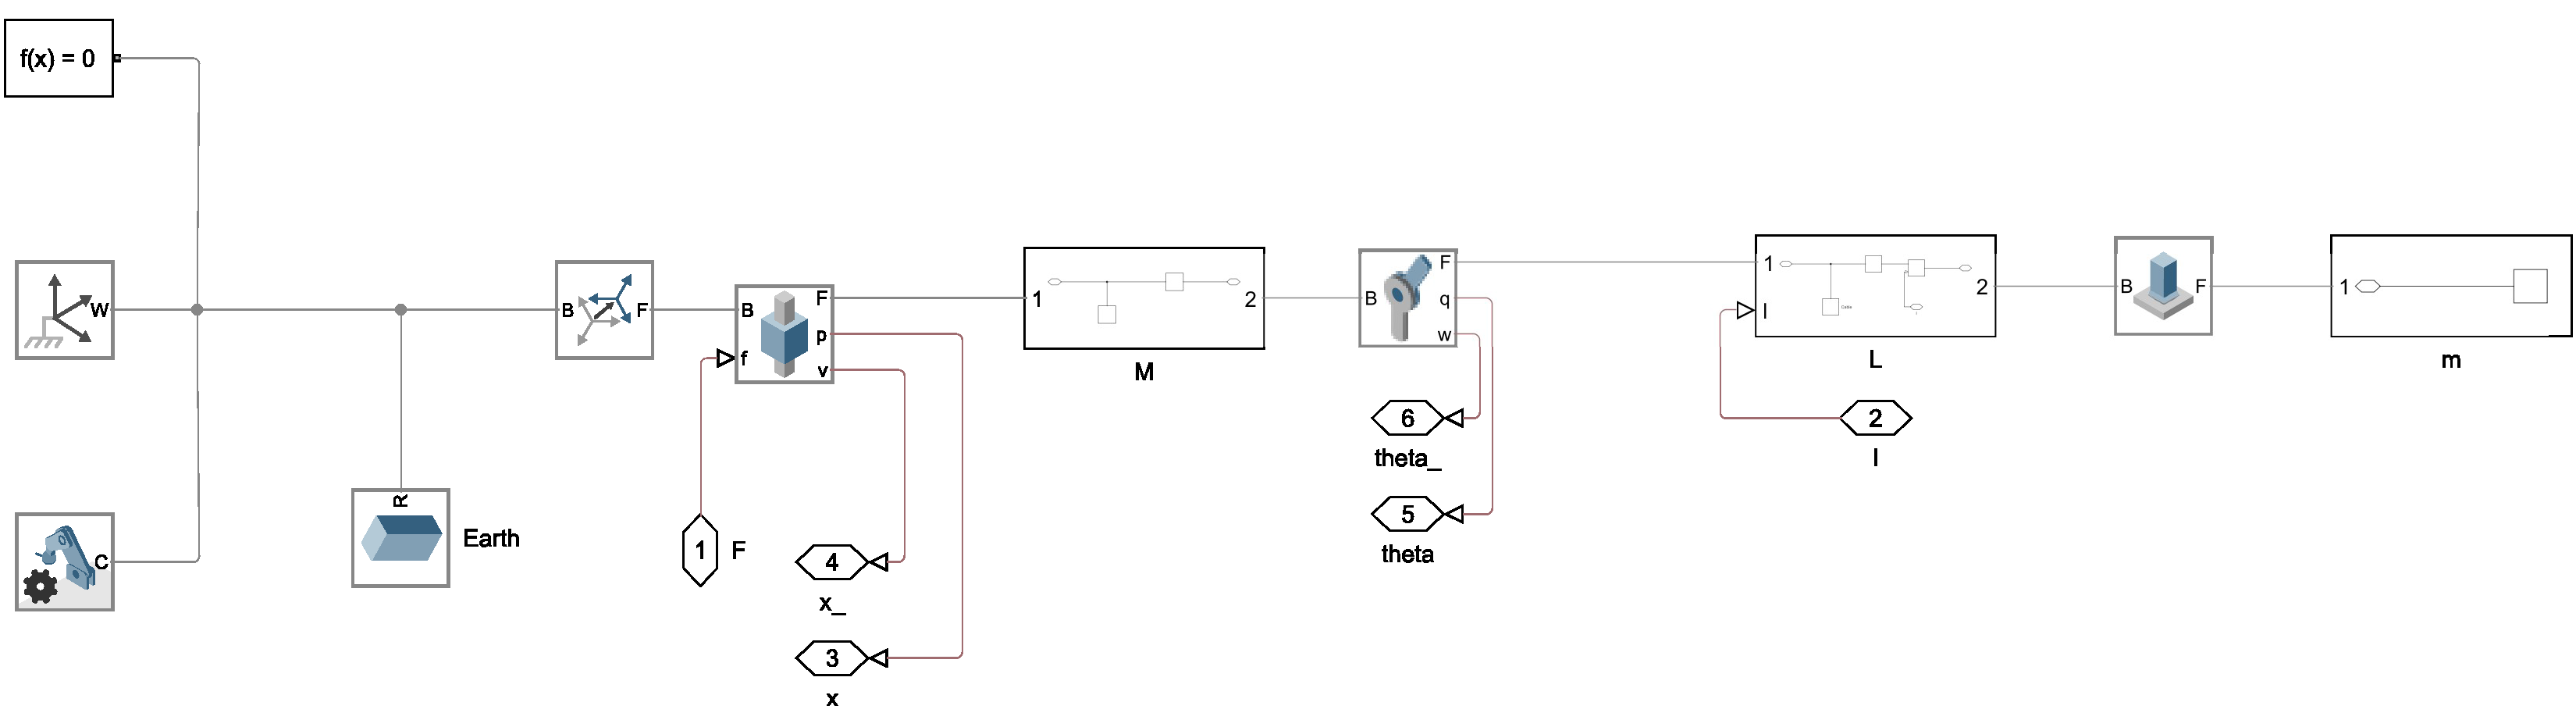
\includegraphics[width=0.9\textwidth]{images/0_System_Modeling/simscape_multibody_plant_detailed.png}
    \caption{معماری داخلی مدل \lr{Simscape Multibody} شامل مفاصل، بلوک‌های فیزیکی و زنجیرهٔ سینماتیکی}
    \label{fig:simscape_detailed}
\end{figure}

\subsection{تفکیک گرافیک از دینامیک در مدل‌سازی کابل}

در معادلات تحلیلی، کابل بدون جرم فرض شده است. برای جلوگیری از بروز خطای محاسباتی ناشی از اعمال ناخواستهٔ جرم و اینرسیِ کابل در شبیه‌ساز، مسیرِ پس از مفصل دورانی به دو شاخهٔ موازی تفکیک شده است:
\begin{enumerate}
    \item \textbf{شاخهٔ دینامیکی:} این مسیر تنها شامل مفصل کشویی و جرم نقطه‌ای آونگ ($m$) است و فاصلهٔ فیزیکی بار را به عنوان یک متغیر وابسته به زمان تعیین می‌کند.
    \item \textbf{شاخهٔ بصری (\lr{Visual}):} این مسیر صرفاً شامل هندسهٔ کابل جهت رندرینگ در محیط سه‌بعدی است و به دلیل نداشتنِ خواص اینرسی، هیچ‌گونه تأثیری بر معادلات حرکت سیستم نخواهد داشت.
\end{enumerate}

\subsection{پیکربندی ورودی‌های سینماتیکی کابل}

از آنجا که سیستم بر پایهٔ کنترل طول کابل عمل می‌کند، حالتِ مفصل کشوییِ متصل به بار، بر روی گزینهٔ دریافت از ورودی (\lr{Provided by Input}) تنظیم شده است. برای جلوگیری از بروز خطای کمبود مشتقات (\lr{Derivative Starvation}) در محاسبات عددی، بلوک \lr{Plant} به گونه‌ای پیکربندی شده است که درگاه ورودی کابل، مجموعهٔ کامل سیگنال‌های سینماتیکی شامل موقعیت $l$، سرعت $\dot{l}$ و شتاب $\ddot{l}$ را هم‌زمان از کنترل‌کننده دریافت کند.

تأمین پیوستهٔ این سه سیگنال تضمین می‌کند که نیروهای وابسته به سرعت و شتاب (مانند نیروهای کوریولیس و اینرسی) توسطِ حل‌گر \lr{Simscape} با دقت کامل و بدون نیاز به مشتق‌گیری‌های عددیِ ناپایدار محاسبه شوند.